\documentclass[10pt,A4paper]{article}
\usepackage[utf8]{inputenc}
\usepackage[T2A]{fontenc}
\usepackage[russian,english]{babel}
\usepackage{amsmath,amsfonts,amssymb,euscript,graphicx,wrapfig,multirow}
\usepackage{dsfont}
\usepackage{amsthm}
\inputencoding{utf8}
%\bibliographystyle{unsrt}


\usepackage{geometry} % Меняем поля страницы.
\geometry{left=1cm}% левое поле
\geometry{right=1cm}% правое поле
\geometry{top=1cm}% верхнее поле
\geometry{bottom=1.5cm}% нижнее поле


%\usepackage[backend=biber,style=gost-numeric,sorting=none]{biblatex}
%\addbibresource{../common/notmy.bib}
%\addbibresource{../common/my.bib}
%\usepackage{../../../biblatex2bibitem/biblatex2bibitem}

\usepackage{hyperref}
\usepackage{cite}

\makeatletter
%\renewcommand{\fnum@figure}{Figure \thefigure}
\renewcommand{\@biblabel}[1]{#1.}
\makeatother

\newcommand{\Definition}[1]{\smallskip{\sc Definition#1.}}



\sloppy \textheight = 230mm \textwidth = 155mm \topmargin = -3mm
\oddsidemargin=3mm \evensidemargin=4pt

\begin{document}
%\renewcommand\refname{\centering References}


% Переключаем язык на английский.
% Очень полезно как в плане типографики (в том числе расстановки переносов),
% так и в плане того, что не надо переименовывать "Рисунок" в "Figure"
\selectlanguage{english}


\title{
	Particular examples of planar integral point sets and their classification
	\footnote{
		This work was carried out at Voronezh State University and supported by the Russian Science
		Foundation grant 19-11-00197.
	}
}

\author{
	Avdeev N.N.
	\footnote{nickkolok@mail.ru, avdeev@math.vsu.ru}
	, Momot E.A., Zvolinskiy A.E.
	\\
	\\
	\emph{Voronezh State University}
}

\maketitle


To the blessed memory of Professor Semën Samsonovich Kutateladze
% Я взял такое написание с
% https://mathscinet.ams.org/mathscinet/MRAuthorID/197072
% и никоим образом на нём не настаиваю



\paragraph{Abstract.}

A planar integral point set (PIPS) is a finite set of non-collinear points in the Euclidean plane
such that the Euclidean distance between any pair of points is an integer.
These sets are characterized by their cardinality (the finite number of points),
diameter (the maximum pairwise distance), and characteristic (the smallest positive integer \(q\)
such that all triangular areas are commensurable with \(\sqrt{q}\)).
The characteristic remains invariant under translations, dilations, reflections, and even the addition or removal of points.

Existing classifications include sets in semi-general position (no three points collinear)
and general position (no three collinear and no four concyclic).
Circular sets and facher sets (all but one point on a line) are prominent examples,
but finding sets in general position is challenging; for instance, the largest known set has seven points,
and no eight-point example is currently known.

This work introduces new examples to advance the classification, including rails sets (points on two parallel lines)
and sets with multiple symmetries.
We also present sets with many shared points that cannot be merged.
These constructions highlight the potential of sequential extensions and limitations of merging sets,
offering insights into the structure and properties of planar integral point sets.


\paragraph{Аннотация.}

Плоское целоудалённое множество есть конечное множество точек на евклидовой плоскости,
не содержащееся ни в какой прямой,
такое что евклидово расстояние между любой парой точек является целым числом.
Эти множества характеризуются своей мощностью (конечным числом точек),
диаметром (максимальным попарным расстоянием) и характеристикой (наименьшим положительным целым числом \(q\),
таким что площади всех треугольников, образованных точками множества, соизмеримы с \(\sqrt{q}\)).
Характеристика инвариантна относительно при сдвига, растяжения, отражения, а также добавления или удаления точек.

Существующие классификации включают множества в полуобщем положении (никакие три точки не лежат на одной прямой)
и в общем положении (никакие три точки не лежат на одной прямой и никакие четыре не лежат на одной окружности).
Классическими примерами являются круговые множества и веерные множества (все точки, кроме одной, лежат на одной прямой),
однако нахождение множеств общего положения представляет значительные трудности;
например, наибольшее известное множество имеет семь точек, и пока не найдено множество из восьми точек общего положения.

В данной работе представлены новые примеры для развития классификации,
включая рельсовые множества (точки на двух параллельных прямых),
множества с несколькими симметриями и стреловидные конфигурации.
Мы также рассматриваем множества с большим количеством общих точек, которые нельзя объединить.
Эти конструкции подчёркивают потенциал последовательных растяжений и ограничения на объединение множеств,
демонсnрируя новые особенности структуры и свойств плоских целоудалённых множеств.


\paragraph{Keywords.}
	integral point set,
	classification of planar integral point sets,
	discrete geometry,
	combinatorial geometry


\paragraph{Ключевые слова.}
	целоудалённое множество,
	классификация плоских целоудалённых множеств,
	дискретная геометрия,
	комбинаторная геометрия


Некоторые примеры плоских целоудалённых множеств и их классификация


UDC 519.146 + 514.11

MSC 52C10



\section{Introduction}



\Definition{ 1}\label{dfn1}
	A planar integral point set (PIPS) is a set $\mathcal{P}$
	of non-collinear points in the plane $\mathbb{R}^{2}$ such that
	for any pair of points $P_{1}, P_{2} \in \mathcal{P}$
	the Euclidean distance $|P_{1}P_{2}|$
	between points $P_{1}$ and $P_{2}$ is an integer.


How do we describe a planar integral point set?
For example, by the number of points in it, which is always finite~\cite{anning1945integral,erdos1945integral}
and is said to be the \emph{cardinality} of the PIPS.
Furthermore, we can naturally
define the diameter of a finite point set.

\Definition{ 2}
	The diameter of a planar integral point set $\mathcal{P}$ is defined as
	$
		\operatorname{diam(\mathcal{P})} = \underset{P_{1}, P_{2} \in
		\mathcal{P}}{\max} |P_{1}P_{2}|
		.
	$



\Definition{ 3}(\cite{kemnitz1988punktmengen,kurz2005characteristic})
	The characteristic of a planar integral point set $M$ is the least positive integer $q$
	such that the area of any triangle with vertices $M_1, M_2, M_3 \in M$
	is commensurable with $\sqrt{q}$.

The characteristic of a PIPS does not change if the set is moved, dilated or flipped;
moreover, even addition or deletion of a point does not change the characteristic of a PIPS.


While the minimal possible diameter for planar integral point sets of a given cardinality was being computed,
it was noticed~\cite{kurz2008minimum} that such a diameter is attained at sets with many points on a straight line;
for some estimations on this tendency, we also refer the reader to~\cite{solymosi2003note};
(For the recently established connection between the characteristic and the minimal possible diameter,
see~\cite{avdeev-lushina2025australas}.)
Thus, the following classification was introduced:

\Definition{ 4}
	A PIPS $M$ is said to be in \emph{semi-general position}
	if no three points of $M$ are located in a straight line.


The most dominating examples of PIPSs in semi-general position are circular sets.

\Definition{ 5}
	A planar integral point set that is situated on a circle is said to be a \textit{circular}
	point set.


So, the following constraint appeared.

\Definition{ 6}
	A planar integral point set $M$ is said to be in \emph{general position}
	if no three points of $M$ are located on a straight line
	and no four points of $M$ are located on a circle.


Planar integral point sets in general position are very difficult to find;
the first known examples of such sets with cardinality 7 were presented in~\cite{kreisel2008heptagon}.
Currently, there is no known example of a PIPS of cardinality 8 in general position.

The main purpose of this work is to provide examples of planar integral point sets
that may provide clues for the development of further classification.

It is rather common for points of a PIPS to have non-integer coordinates;
for convenience, in such cases
we use the notation \cite{our-ped-2018,our-pmm-2018,our-vmmsh-2018-translit}:
$\sqrt{p}/q * \{ (x_1;y_1); ...;$ $ (x_n; y_n)  \}$,
which means that each abscissa is multiplied by $1/q$
and each ordinate is multiplied by $\sqrt{p}/q$,  i.e.
\begin{equation}
	\label{eq:char_lattice}
	\sqrt{p}/q * \{ (x_1;y_1); ...; (x_n; y_n)  \}
	=
	\left\{ \left(\frac{x_1}{q};\frac{y_1\sqrt{p}}{q}\right); ...; \left(\frac{x_n}{q};   \frac{y_n\sqrt{p}}{q}\right)  \right\}
	.
\end{equation}
Here $p$ is the characteristic of the PIPS;
any PIPS can be written in this form~\cite[Theorem 4]{our-vmmsh-2018-translit}.

Note that all examples that are discussed below are
located on a union of at most three straight lines.
%In the most pictures these lines are shown as solid lines.
For the classification of PIPSs that are located on a union of two straight lines,
we refer the reader to~\cite{avdeev2019particular}.

There are some examples of PIPSs that are not contained in the union of any three straight lines:
for example, these include the heptagons presented in~\cite{kreisel2008heptagon} and 7-clusters from~\cite{kurz2013constructing}.
However, we have to keep in mind that circular inversion under certain conditions
translates a planar integral point set into a planar integral point set
(although sometimes additional dilation is necessary).
On the other hand, circular inversion may translate a straight line into a circle and vice versa.
Thus, we can consider \emph{generalized circles}, which are circles or straight lines;
obviously, from that point of view all the examples from~\cite{kreisel2008heptagon} and~\cite{kurz2013constructing}
are located on a union of three generalized circles,
because any seven points are located on a union of a circle and two straight lines.




\section{Rails sets}

\Definition{ 7}
	A planar integral point set of $n$ points with $n-1$ points on a straight line is called
	a \textit{facher} set.

Facher sets are predominant examples of planar integral point sets~\cite{zvolinskyR2021facher}.
In~\cite{antonov2008maximal}, facher sets of characteristic 1 are called \textit{semi-crabs}.
%For $9 \leq n \leq 122$, the diameter $d(2,n)$ is reached on a facher point set~\cite{kurz2008minimum}.

\Definition{ 8}[\cite{avdeev2019particular}]
	A non-facher planar integral point set situated on two parallel straight lines
	is called a \textit{rails} set.


Among rails sets, sets with 2 points on one line and all the others on another line dominate.


The two PIPSs below have been obtained by dilating~\cite[Fig. 34]{avdeev2019particular} by $23$ and $29$ respectively;
the third one has been constructed by dilation and merging.



\begin{figure}[h!]
\center{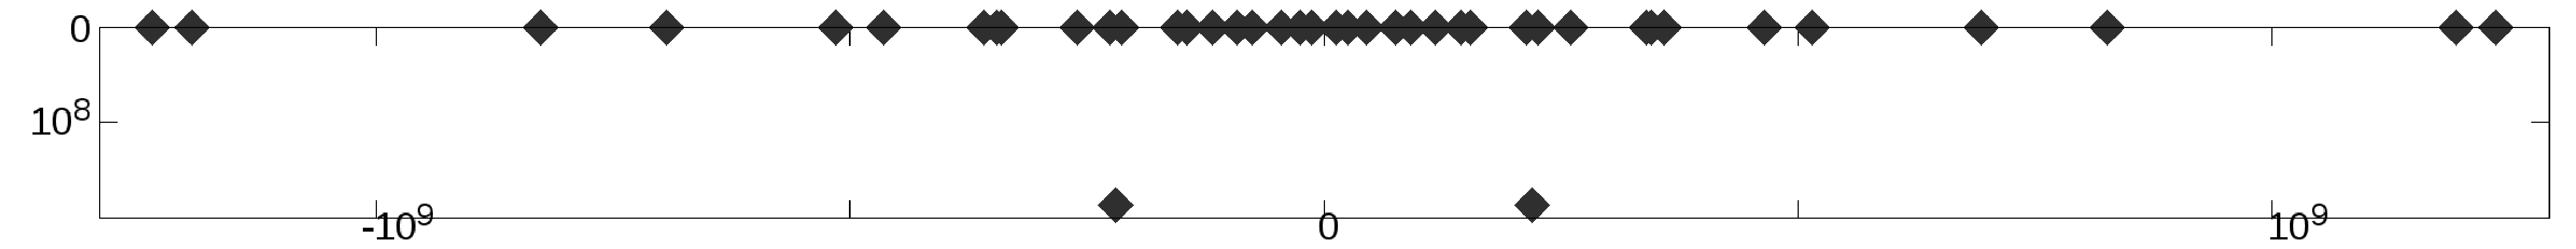
\includegraphics[width=1\linewidth]{./img/42_symm.eps}}
\parbox{1\linewidth}{\caption{A PIPS of cardinality 42 and diameter 2473117504}
\label{42_symm.eps}}
\end{figure}

\begin{figure}[h!]
\center{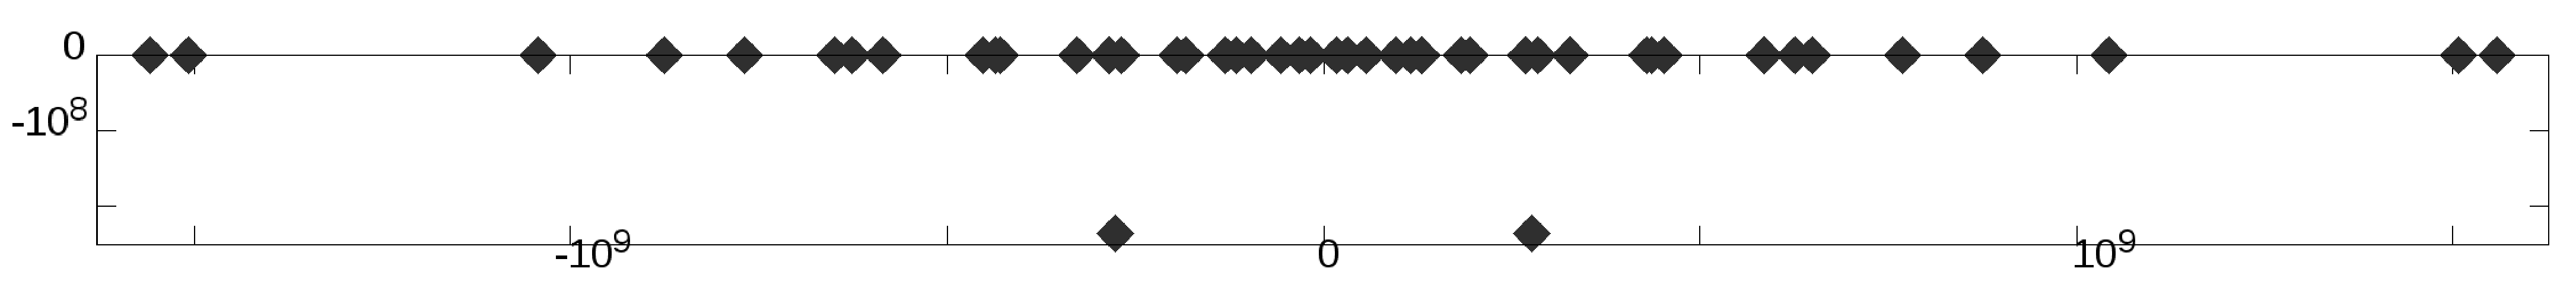
\includegraphics[width=1\linewidth]{./img/46_symm.eps}}
\parbox{1\linewidth}{\caption{A PIPS of cardinality 46 and diameter 3118278592}
\label{46_symm.eps}}
\end{figure}

\begin{figure}[h!]
\center{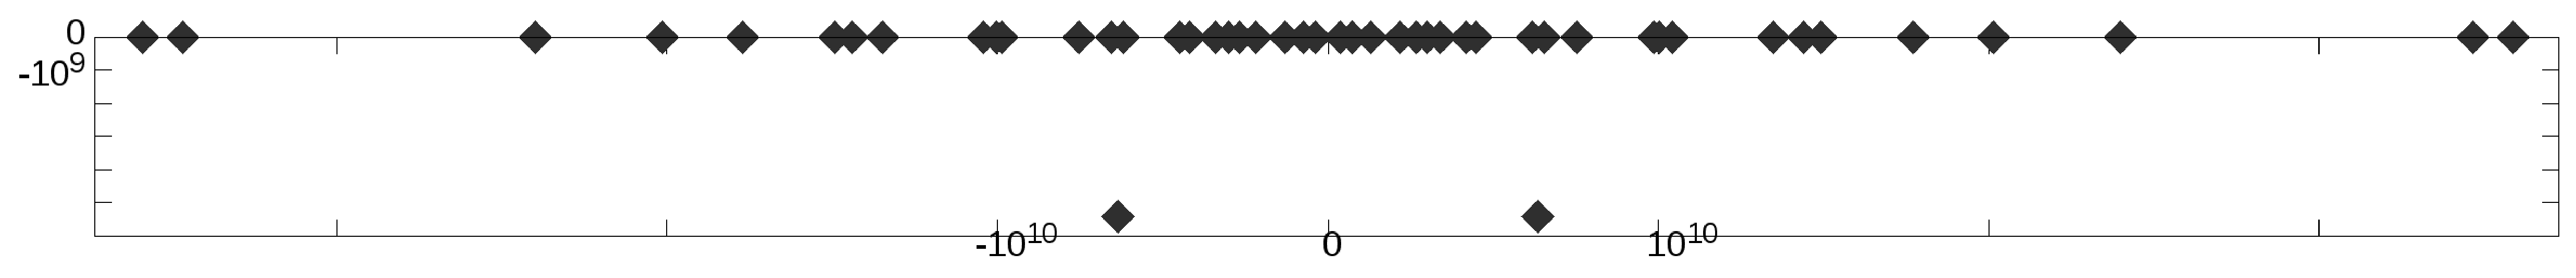
\includegraphics[width=1\linewidth]{./img/48_symm.eps}}
\parbox{1\linewidth}{\caption{A PIPS of cardinality 48 and diameter 71720407616}
\label{48_symm.eps}}
\end{figure}

\begin{itemize}
\setlength{\itemsep}{-1mm}


\item
Figure~\ref{42_symm.eps}:
\begin{multline*}
	\mathcal{P}_{42}=\sqrt{154}/{1} * \{
		(\pm219513840; -15069600);
		(\pm 345596160; 0);
		(\pm260201760; 0);
		\\
		(\pm225792840; 0);
		(\pm213234840; 0);
		(\pm153961080; 0);
		(\pm144668160; 0);
		(\pm25116000; 0);
		\\
		(\pm694026840; 0);
		(\pm514710560; 0);
		(\pm359116940; 0);
		(\pm13423904; 0);
		(\pm75682880; 0);
		\\
		(\pm464143680; 0);
		(\pm827069880; 0);
		(\pm92144325; 0);
		(\pm1195180740; 0);
		(\pm1236558752; 0);
		\\
		(\pm44590560; 0);
		(\pm339925740; 0);
		(\pm117312468; 0)
	\}
\end{multline*}

\item
Figure~\ref{46_symm.eps}:
\begin{multline*}
	\mathcal{P}_{46}=
	\sqrt{154}/{1} * \{
		(\pm276778320; -19000800);
		(\pm435751680; 0);
		(\pm328080480; 0);
		\\
		(\pm268861320; 0);
		(\pm194124840; 0);
		(\pm182407680; 0);
		(\pm1559139296; 0);
		(\pm284695320; 0);
		\\
		(\pm1506967020; 0);
		(\pm1042827240; 0);
		(\pm875077320; 0);
		(\pm648982880; 0);
		(\pm585224640; 0);
		\\
		(\pm452799620; 0);
		(\pm95426240; 0);
		(\pm16925792; 0);
		(\pm116181975; 0);
		(\pm428602020; 0);
		\\
		(\pm56222880; 0);
		(\pm769560480; 0);
		(\pm626458560; 0);
		(\pm31668000; 0);
		(\pm130761918; 0)
	\}
\end{multline*}

\item
Figure~\ref{48_symm.eps}:
\begin{multline*}
	\mathcal{P}_{48}=
	\sqrt{154}/{1} * \{
		( \pm6365901360 ; -437018400);
		\\
		( \pm10022288640; 0);
		( \pm23985026520 ; 0);
		( \pm389293216 ; 0);
		( \pm6183810360 ; 0);
		\\
		( \pm4464871320 ; 0);
		( \pm4195376640 ; 0);
		( \pm728364000 ; 0);
		( \pm35860203808 ; 0);
		( \pm34660241460 ; 0);
		\\
		( \pm7545851040 ; 0);
		( \pm20126778360 ; 0);
		( \pm14926606240 ; 0);
		( \pm13460166720 ; 0);
		( \pm10414391260 ; 0);
		\\
		( \pm2194803520 ; 0);
		( \pm2672185425 ; 0);
		( \pm9857846460 ; 0);
		( \pm1293126240 ; 0);
		( \pm17699891040 ; 0);
		\\
		( \pm14408546880 ; 0);
		( \pm3007524114 ; 0);
		( \pm6547992360 ; 0);
		( \pm3402061572 ; 0)
	\}
\end{multline*}

\end{itemize}

Taking these examples into consideration,
we can conjecture that there is an infinite point set with rational distances
that contains $\mathcal{P}_{48}$.
(However, it is known~\cite{solymosi2010question} that
if a point set $S$ with rational distances has infinitely many points on a line or on a circle,
then all but 4 and 3 points, respectively, of $S$ are on the line or on the circle.)


\section{Example of sets with many common points that cannot be merged}

Figure~\ref{8_with_many_common} shows an example of three PIPSs of cardinality 8,
each pair of which shares 6 or 7 points but cannot be combined into another PIPS.

\begin{figure}[h!]
	\begin{minipage}[h]{0.32\linewidth}
		\begin{center}
			\includegraphics[width=1\linewidth]{./img/8_2520_143_symm1.eps}\\ a)
		\end{center}
	\end{minipage}
	\hfill
	\begin{minipage}[h]{0.32\linewidth}
		\begin{center}
			\includegraphics[width=1\linewidth]{./img/8_2520_143_symm2.eps}\\ b)
		\end{center}
	\end{minipage}
	\begin{minipage}[h]{0.32\linewidth}
		\begin{center}
			\includegraphics[width=1\linewidth]{./img/8_2520_143_4a27_other.eps}\\ c)
		\end{center}
	\end{minipage}
	\hfill
	\caption{PIPSs with cardinality 8 and diameter 2520 with many common points}
	\label{8_with_many_common}
\end{figure}

\begin{itemize}
\item
$\mathcal{P}=\sqrt{143}/2*\{
( \pm1620 ; 0);
( \pm1920 ; 300);
( \pm735 ; 75);
( \pm340 ; 0)
\}$

\item
$\mathcal{P}=\sqrt{143}/2*\{
( \pm1620 ; 0);
( \pm1920 ; 300);
( \pm735 ; 75);
( \pm1767 ; 147)
\}$

\item
$\mathcal{P}=
\sqrt{143}/2*\{
( \pm1620 ; 0);
( \pm1920 ; 300);
( \pm735 ; 75);
( -340 ; 0);
( 1767 ; 147)
\}$

\end{itemize}

The distance between the non-adoptable points is
$
	\sqrt{\left(\frac{1767}{2} - \frac{340}{2}\right)^2 + \left(\frac{147}{2}\right)^2\cdot143} = 2\sqrt{320401}
$.
Notably, 320401 is a prime.

\section{Integral point sets with two axes of symmetry}

The set $\mathcal{P}_{19}$ shown in Figure~\ref{19_20663808074} was obtained from the set $\mathcal{P}_{9}$ shown in Figure~\ref{9_2890_1_02e6af}
by dilation and looking for points on the $x$ axis.


\begin{figure}[h!]
\center{\includegraphics[width=1\linewidth]{./img/9_2890_1_02e6afb1c19846c6c4debb44e52cc468_other.eps}}
\parbox{1\linewidth}{\caption{A PIPS of cardinality 9 and diameter 2890}
\label{9_2890_1_02e6af}}
\end{figure}

\begin{equation}
	\mathcal{P}_9=\{
	( 0 ; 0);
	( \pm1445 ; 0);
	( \pm1085 ; 0);
	( -455 ; \pm528);
	( 455 ; \pm528)
	\}
\end{equation}

\begin{figure}[h!]
\center{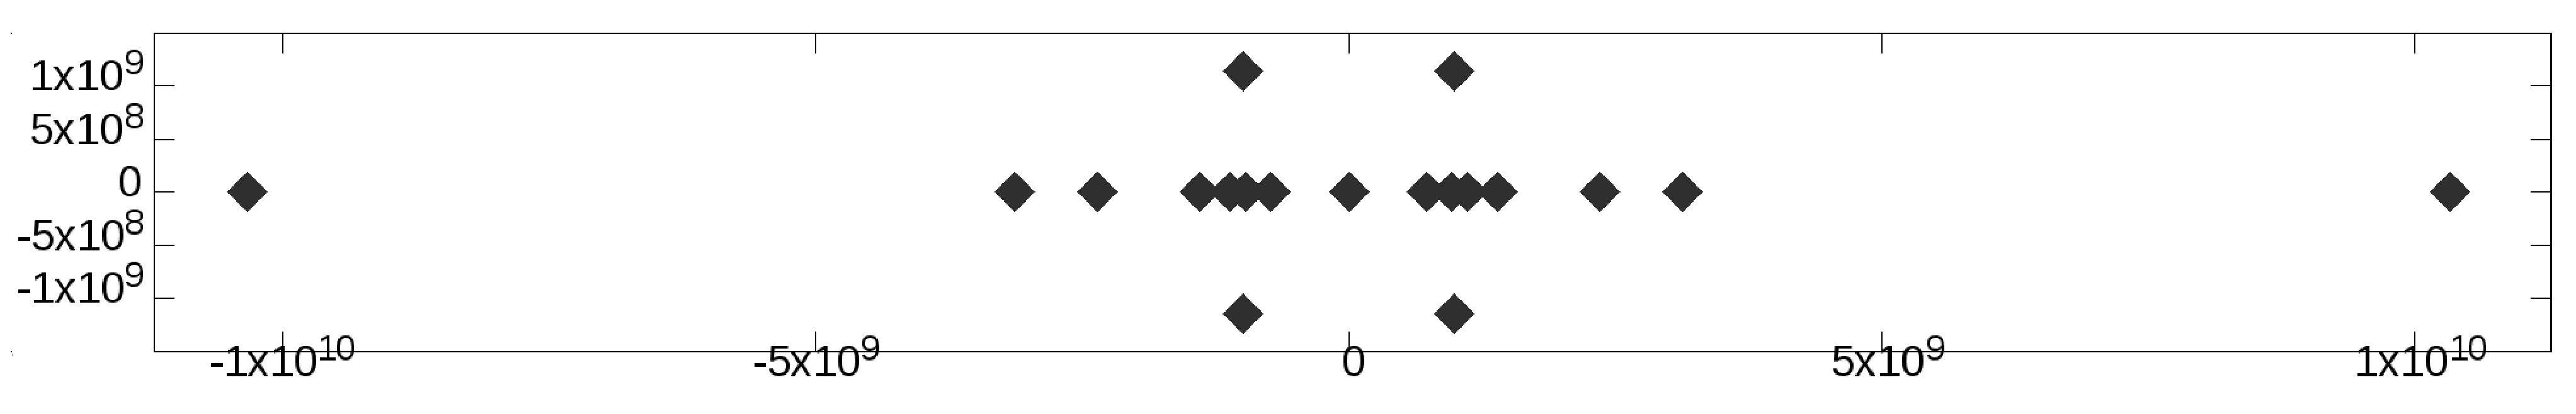
\includegraphics[width=1\linewidth]{./img/19_20663808074_1_0070b97f26bb194a7de2ddc37ee38b08_symm.eps}}
\parbox{1\linewidth}{\caption{A PIPS of cardinality 19 and diameter 20663808074}
\label{19_20663808074}}
\end{figure}

\begin{multline*}
	\mathcal{P}_{19}=
	\{
		( 0 ; 0);
		( -987843675 ; \pm1146332880);
		( 987843675 ; \pm1146332880);
		\\
		( \pm729918777 ; 0);
		( \pm972103809 ; 0);
		%\\
		( \pm1113030324 ; 0);
		( \pm1400170149 ; 0);
		\\
		( \pm3137217825 ; 0);
		( \pm2355627225 ; 0);
		( \pm10331904037 ; 0)
	\}
\end{multline*}

\section{Arrow-like planar integral point sets with one axis of symmetry}

In Figure~\ref{17_1024296_1_639b}, the following PIPS is shown:
\begin{multline*}
	\mathcal{P}_{17}=
	\{
		( -2847 ; \pm72072);
		( 47073 ; \pm124488);
		( 47073 ; 0);
		( \pm98943 ; 0);
		%\\
		( -694668 ; 0);
		( 15457 ; 0);
		\\
		( -71487 ; 0);
		( -50367 ; 0);
		%\\
		( -14943 ; 0);
		%\\
		( 23582 ; 0);
		( 63073 ; 0);
		( 125307 ; 0);
		( 172207 ; 0);
		( 329628 ; 0)
	\}
\end{multline*}
Note that the axis of symmetry for $\mathcal{P}_{17}$ is the $x$ axis;
all such sets are of characteristic 1.
Moreover, note that the set contains three points with the same first coordinates.

\begin{figure}[h!]
\center{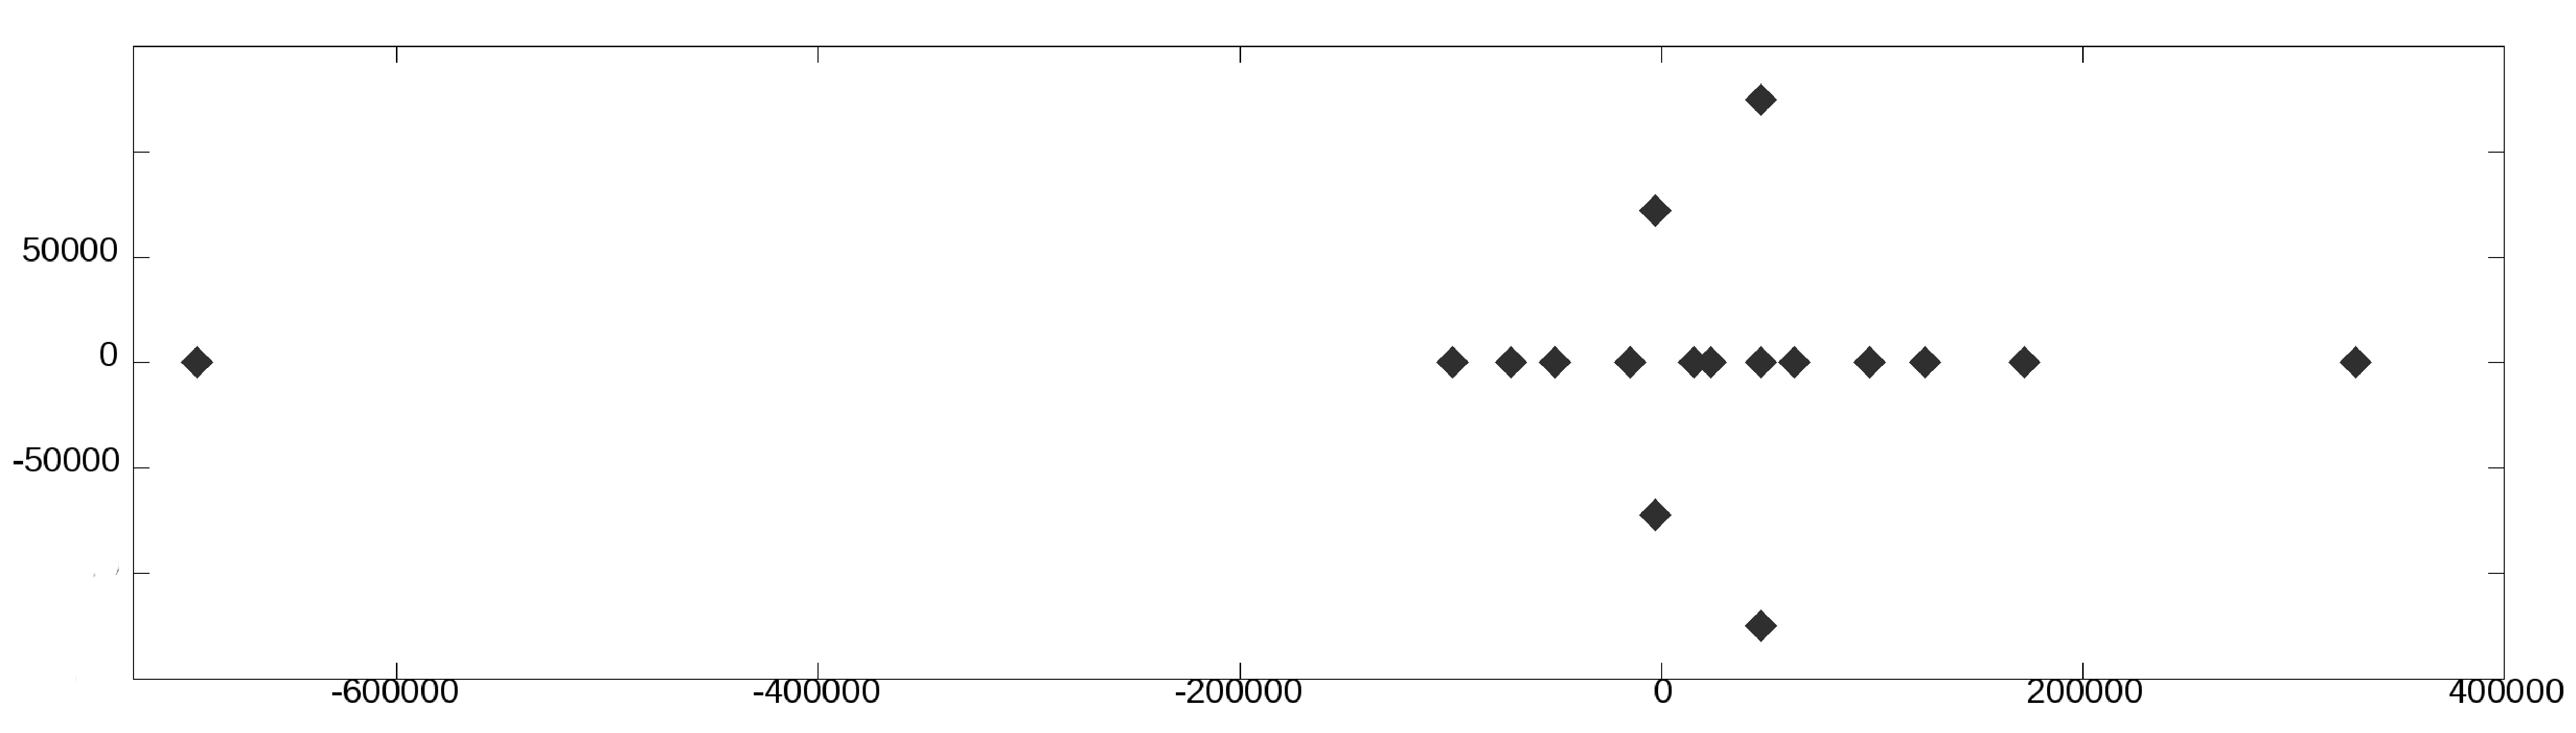
\includegraphics[width=1\linewidth]{./img/17_1024296_1_639b7a0452227fde1aceabf02e8778e4_other.eps}}
\parbox{1\linewidth}{\caption{A PIPS of cardinality 17 and diameter 1024296}
\label{17_1024296_1_639b}}
\end{figure}

In Figures~\ref{10_2431_1_0606} and~\ref{15_19203744_1_80db}, other examples of arrow-like PIPSs are shown.
The one in Figure~\ref{15_19203744_1_80db} is obtained from the one in Figure~\ref{10_2431_1_0606}
by dilation and looking for points on the $x$ axis.




\begin{figure}[h!]
	\center{\includegraphics[width=1\linewidth]{./img/10_2431_1_0606659e825917be0c3c431c1375bf21_other.eps}}
	\parbox{1\linewidth}{\caption{A PIPS of cardinality 10 and diameter 2431}
	\label{10_2431_1_0606}}
\end{figure}


\begin{figure}[h!]
	\center{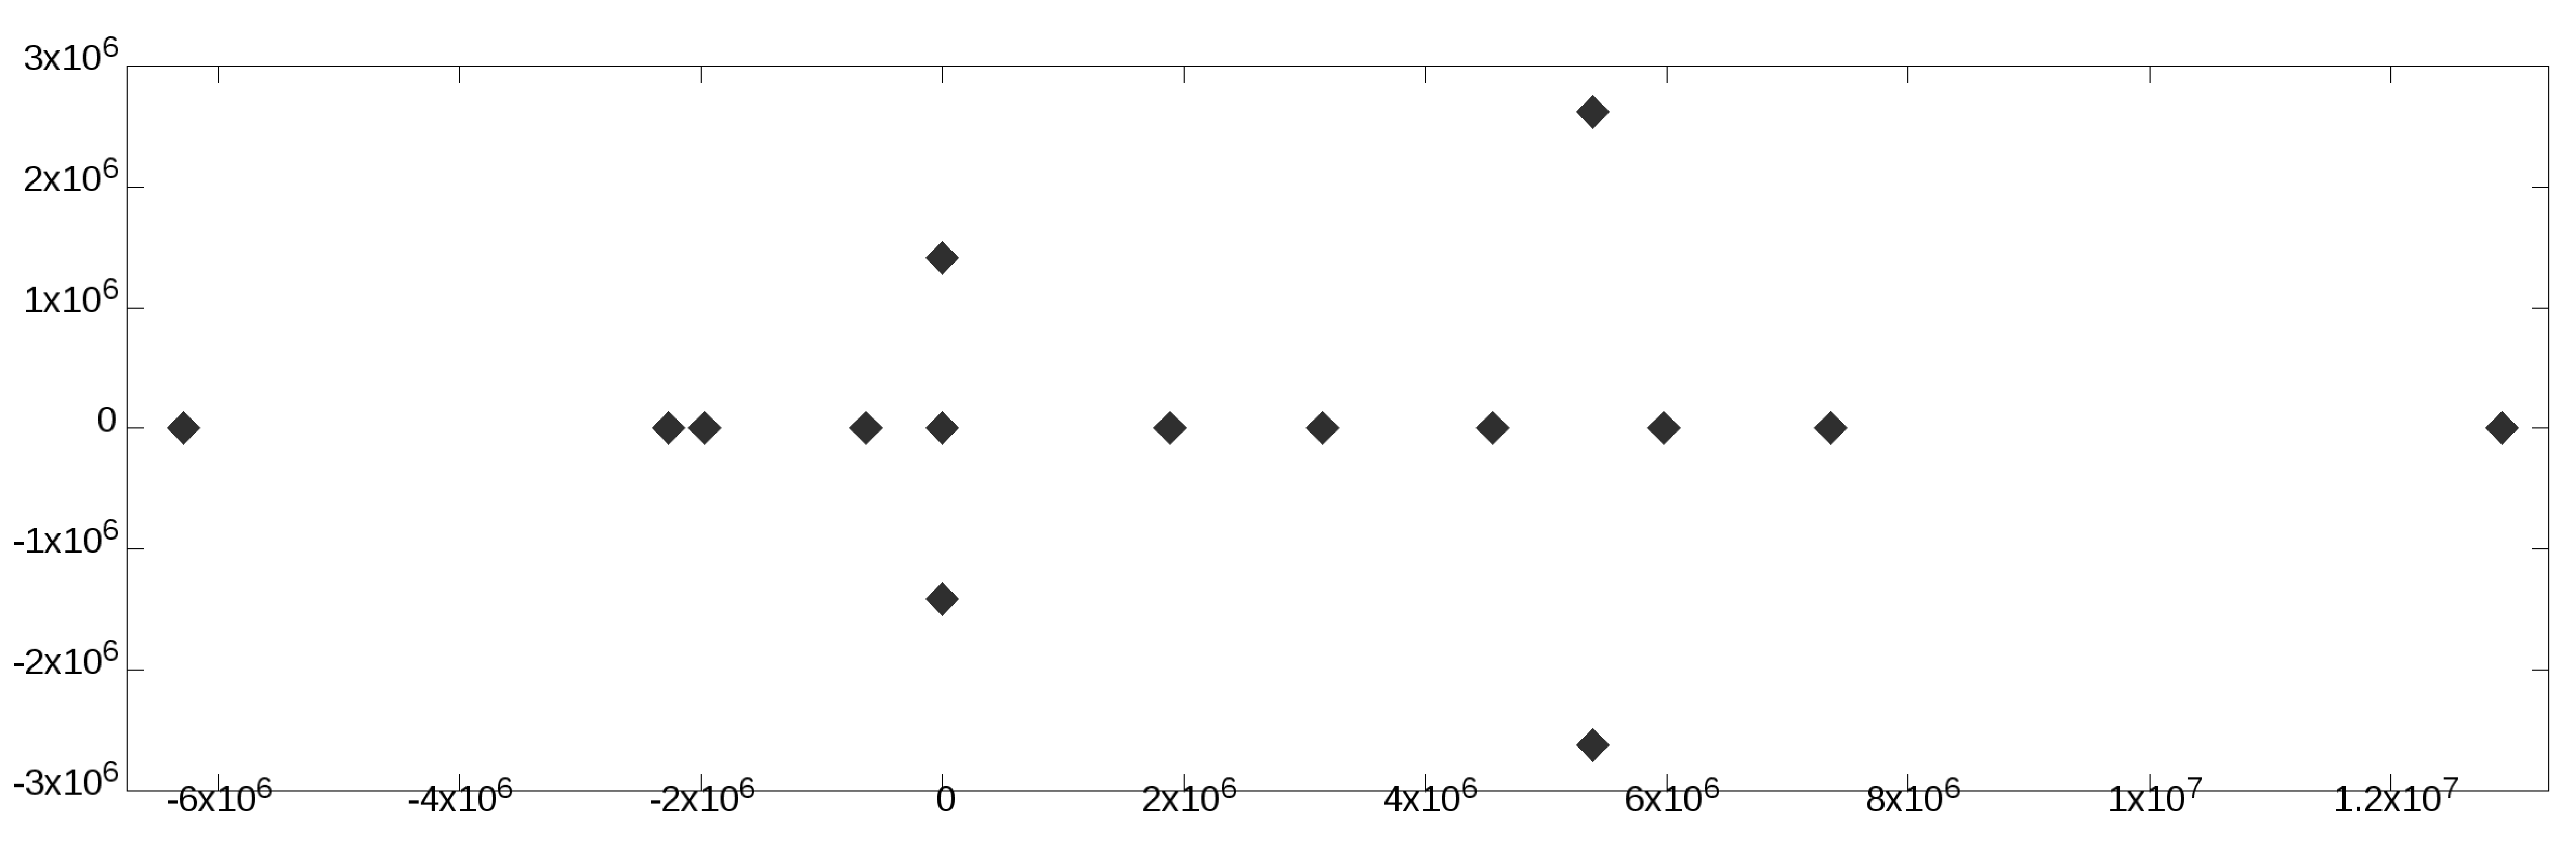
\includegraphics[width=1\linewidth]{./img/15_19203744_1_80dbf8e05b25f69b8366e50d1d7463f6_other.eps}}
	\parbox{1\linewidth}{\caption{A PIPS of cardinality 15 and diameter 19203744}
	\label{15_19203744_1_80db}}
\end{figure}

Figure~\ref{10_2431_1_0606}:
\begin{equation*}
	\mathcal{P}_{10} =
	\{
		( 0 ; 0);
		( 0 ; \pm252);
		( 960 ; \pm468);
		( -1120 ; 0);
		( -405 ; 0);
		( 336 ; 0);
		( 561 ; 0);
		( 1311 ; 0)
	\}
\end{equation*}

Figure~\ref{15_19203744_1_80db}:
\begin{multline*}
	\mathcal{P}_{15} =
	\{
		( 0 ; 0);
		( 0 ; \pm1413720);
		( 5385600 ; \pm2625480);
		\\
		( -6283200 ; 0);
		( -2272050 ; 0);
		( -1971915 ; 0);
		( -635040 ; 0);
		( 1884960 ; 0);
		\\
		( 3147210 ; 0);
		( 4558176 ; 0);
		( 5976333 ; 0);
		( 7354710 ; 0);
		( 12920544 ; 0)
	\}
\end{multline*}



\section{Other examples}

Figure~\ref{8_2535_1_d680} displays a PIPS with
no axis of symmetry;
although the set is of characteristic 1,
it cannot be extended by the reflection in the $x$-axis.
Moreover, we failed to extend it by dilation and looking for extra points on the $x$-axis.

\begin{multline*}
	\mathcal{P}_8=
	\sqrt{1}/13*
	\{
	( 0 ; 0);
	( 8450 ; 0);
	( 12844 ; 0);
	( 21294 ; 0);
	( 29575 ; 0);
	\\
	( -2366 ; -8112);
	( 10647 ; -14196);
	( 15022 ; -3696)
	\}
\end{multline*}
%
\begin{figure}[h!]
\center{\includegraphics[width=0.9\linewidth]{./img/8_2535_1_other.eps}}
\parbox{1\linewidth}{\caption{A PIPS of cardinality 8 and diameter 2535}
\label{8_2535_1_d680}}
\end{figure}

The set shown in Figure~\ref{8_2400_42_56f3} has an axis of symmetry, but it is the $y$-axis, not the $x$-axis.
Due to the fact that its characteristic is not 1,
the set cannot be rotated by $90^\circ$ but still be on the lattice~\eqref{eq:char_lattice}:
\begin{equation*}
	\mathcal{P}_{8y}=
	\sqrt{42}/1*\{( \pm1200 ; 0);
	( \pm529 ; 182);
	( \pm814 ; 152);
	( \pm440 ; 80)
	\}
\end{equation*}

\begin{figure}[h!]
	\center{\includegraphics[width=0.9\linewidth]{./img/8_2400_42_symm.eps}}
	\parbox{1\linewidth}{\caption{A PIPS of cardinality 8 and diameter 2400}
	\label{8_2400_42_56f3}}
\end{figure}



\section{Final remarks}
All given planar integral point sets were obtained through a combination of computer search and the authors' intuition.

The source code can be obtained at https://gitlab.com/Nickkolok/ips-algo

\section{Acknowledgements}
The authors thank Dr. Prof. E.M. Semenov and Dr.~A.S.~Usachev for proofreading.
Also the authors owe special thanks to the anonymous referee
for the helpful comments and suggestions on the paper.


A special remark from N. Avdeev:
I would like to express my deepest gratitude to the late Professor Semën Samsonovich Kutateladze,
who played a pivotal role in my scientific career.
He recommended the journal for my first significant scholarly article~\cite{our-mz-rus-translit}
and facilitated its submission, marking the start of a pioneering series of works on this topic at our university.
This contribution is dedicated to his memory.




Авдеев Николай Николаевич

Воронежский государственный университет, кафедра теории функций и геометрии, аспирант

Россия, 394006, г. Воронеж, Университетская пл., 1

E-mail: nickkolok@mail.ru, avdeev@math.vsu.ru


Avdeev Nikolai Nikolaevich

Voronezh State University, Department of Function Theory and Geometry, postgraduate student

Russia, 394006, Voronezh, University sq., 1



Момот Екатерина Александровна

Воронежский государственный университет, кафедра функционального анализа и операторных уравнений, выпускница

Россия, 394006, г. Воронеж, Университетская пл., 1



Momot Ekaterina Alexandrovna

Voronezh State University, Department of Functional Analysis and Operator Equations, graduated from

Russia, 394006, Voronezh, University sq., 1



Зволинский Александр Евгеньевич

Воронежский государственный университет, кафедра теории функций и геометрии, выпускник

Россия, 394006, г. Воронеж, Университетская пл., 1



Zvolinsky Alexandr Evgenievich

Voronezh State University, Department of Function Theory and Geometry, graduated from

Russia, 394006, Voronezh, University sq., 1


\begin{thebibliography}{99}
{}
\bibitem{anning1945integral}
\emph{Anning} \emph{N. H.}, \emph{Erdős} \emph{P.} Integral distances // Bulletin of
the American Mathematical Society. — 1945. — Vol. 51, no. 8. — Pp. 598–600. — DOI: \href
{https://doi.org/10.1090/S0002-9904-1945-08407-9} {\nolinkurl
{10.1090/S0002-9904-1945-08407-9}}.
{}
\bibitem{erdos1945integral}
\emph{Erdős} \emph{P.} Integral distances // Bulletin of the American Mathematical
Society. — 1945. — Vol. 51, no. 12. — P. 996. — DOI: \href
{https://doi.org/10.1090/S0002-9904-1945-08490-0} {\nolinkurl
{10.1090/S0002-9904-1945-08490-0}}.
{}
\bibitem{kemnitz1988punktmengen}
\emph{Kemnitz} \emph{A.} Punktmengen mit ganzzahligen Abständen [Point sets with integral distances]. — 1988. (in German)
{}
\bibitem{kurz2005characteristic}
\emph{Kurz} \emph{S.} On the characteristic of integral point sets in {$\mathbb
{E}^m$} // Australasian Journal of Combinatorics. — 2006. — Vol. 36. — Pp. 241–248. —
arXiv: \href {http://arxiv.org/abs/math/0511704} {\nolinkurl {math/0511704}}.
{}
\bibitem{kurz2008minimum}
\emph{Kurz} \emph{S.}, \emph{Wassermann} \emph{A.} On the minimum diameter of
plane integral point sets // Ars Combinatoria. — 2011. — Vol. 101. — Pp. 265–287. — arXiv:
\href {http://arxiv.org/abs/0804.1307} {\nolinkurl {0804.1307}}.
{}
\bibitem{solymosi2003note}
\emph{Solymosi} \emph{J.} Note on integral distances // Discrete \& Computational
Geometry. — 2003. — Vol. 30, no. 2. — Pp. 337–342. — DOI: \href
{https://doi.org/10.1007/s00454-003-0014-7} {\nolinkurl {10.1007/s00454-003-0014-7}}.{}
\bibitem{avdeev-lushina2025australas}
\emph{Avdeev} \emph{N.}, \emph{Lushina} \emph{E.} On the characteristic and diameter
of planar integral point sets // Australasian Journal of Combinatorics. – 2025. – V. 93. – No. 3. – Pp. 461-477. DOI:
\href {https://doi.org/10.48550/arXiv.2407.08121} {\nolinkurl
{10.48550/arXiv.2407.08121}}. — arXiv: \href {http://arxiv.org/abs/2407.08121} {\nolinkurl
{2407.08121}}
{}
\bibitem{kreisel2008heptagon}
\emph{Kreisel} \emph{T.}, \emph{Kurz} \emph{S.} There are integral heptagons, no three
points on a line, no four on a circle // Discrete \& Computational Geometry. — 2008. —
Vol. 39, no. 4. — Pp. 786–790. — DOI: \href {https://doi.org/10.1007/s00454-007-9038-6}
{\nolinkurl {10.1007/s00454-007-9038-6}}.
{}
\bibitem{our-ped-2018}
\emph{Avdeev N. N.} On integral point sets in special position,
\emph{Nekotorye voprosy analiza, algebry, geometrii i matematicheskogo obrazovaniya:
materialy mezhdunarodnoi molodezhnoi nauchnoi shkoly «Aktual'nye napravleniya matematicheskogo analiza i smezhnye voprosy»}
 — 2018. — Vol. 8. — Pp. 5–6.
{}
\bibitem{our-pmm-2018}
\emph{Avdeev N. N.}
Ob otyskanii tseloudalennykh mnozhestv special'nogo vida
[On the search of special integral point sets],
Aktual'nye problemy prikladnoj matematiki, informatiki i mekhaniki --- sbornik trudov Mezhdunarodnoj nauchnoj konferentsii,
2018. Pp. 492–498. (in Russian)
{}
\bibitem{our-vmmsh-2018-translit}
\emph{Avdeev} \emph{N. N.}, \emph{Semenov} \emph{E. M.}
Mnozhestva tochek s celochislennymi rasstoyaniyami na
ploskosti i v evklidovom prostranstve
[Integral point sets in the plane and Euclidean space],
Matematicheskij forum (Itogi nauki. Yug Rossii).
2018. — Pp. 217–236.
{}
\bibitem{avdeev2019particular}
\emph{Avdeev} \emph{N. N.}, \emph{Zvolinsky} \emph{R. E.},
\emph{Momot} \emph{E. A.} On particular diameter bounds for integral point sets in higher
dimensions
\it{Proceedings of Voronezh State University. Series: Physics. Mathematics}.
2025. — Vol. 1. — Pp. 62–77. —
arXiv: \href {http://arxiv.org/abs/1909.10386} {\nolinkurl {1909.10386}}.
{}
\bibitem{kurz2013constructing}
Constructing $7$-clusters / S. Kurz [et al.] // Serdica Journal of Computing. — 2014. — Vol. 8,
no. 1. — Pp. 47–70. — arXiv: \href {http://arxiv.org/abs/1312.2318} {\nolinkurl {1312.2318}}.
{}
\bibitem{zvolinskyR2021facher}
	Zvolinsky R. E. Facher integral point sets with particular distances of arbitrary cardinality,
	Aktual'nye problemy prikladnoj matematiki, informatiki i mekhaniki --- sbornik trudov Mezhdunarodnoj nauchnoj konferentsii,
	2021. Pp. 668–674.
{}
\bibitem{antonov2008maximal}
\emph{Antonov} \emph{A. R.}, \emph{Kurz} \emph{S.} Maximal integral point sets over
{$\mathbb {Z}^2$} // International Journal of Computer Mathematics. — 2008. — Vol. 87,
no. 12. — Pp. 2653–2676. — DOI: \href {https://doi.org/10.1080/00207160902993636}
{\nolinkurl {10.1080/00207160902993636}}. — arXiv: \href {http://arxiv.org/abs/0804.1280}
{\nolinkurl {0804.1280}}.{}
\bibitem{solymosi2010question}
\emph{Solymosi} \emph{J.}, \emph{De Zeeuw} \emph{F.} On a question of Erdős and
Ulam // Discrete \& Computational Geometry. — 2010. — Vol. 43, no. 2. — Pp. 393–401. —
arXiv: \href {http://arxiv.org/abs/0806.3095} {\nolinkurl {0806.3095}}.
{}
\bibitem{our-mz-rus-translit}
	\emph{Avdeev N.N., Semenov E.M.}
	On the sets of points on the plane with integer-valued distances.
	\emph{Mathematical Notes}, 2016, vol. 100, pp. 743--746.
	https://doi.org/10.1134/S0001434616110110
\end{thebibliography}


\end{document}

